%\documentclass{article}
%\usepackage[utf8]{inputenc}

%\title{M2 Internship : Sparsity and Mass Accretion History of Dark Matter Halos}
%\author{magdy.morshed }
%\date{June 2020}

%\begin{document}

%\maketitle

%\section{Introduction}

%\end{document}

\documentclass[12pt]{article}

\usepackage[utf8]{inputenc}

\title{\textbf{Sparsity and Mass Accretion History of Dark Matter Halos}}
\author{Magdy Morshed\thanks{E-mail: magdy.morshed@ens.fr}}
\date{June 15, 2020}

\usepackage{siunitx}
\usepackage{graphicx}
\usepackage{geometry}
\usepackage{amsmath, amscd, amstext, amsbsy, amsopn, amsthm, amsxtra, upref}
\usepackage{amsfonts, amssymb, euscript, eufrak}
\geometry{textwidth = 530pt}
\geometry{textheight = 650pt}
\setlength{\parindent}{4em}
\setlength{\parskip}{1.5em}


\usepackage[T1]{fontenc}
\usepackage{mathabx}
\usepackage{dblfloatfix}
\DeclareSIUnit \h {\ensuremath{\mathit{h}}}
\DeclareSIUnit \parsec {pc}
\DeclareSIUnit \lightyear {ly}

\setlength\parindent{0pt}

\begin{document}

\maketitle

\begin{abstract}
Dark matter halos are cosmic structures in the universe whose densities are described by cosmological perturbations of the cosmic density of the universe. We propose to perform a complete study of the different models.
\end{abstract}

Supervisor : Pier-Stefano Corasaniti

\newpage

\tableofcontents

\newpage

\section*{Introduction : General Framework for Cosmology}

The modern depiction of the evolution of the universe is currently given by the $\Lambda -CDM$ model, the current cosmology (cosmological ?) paradigm. This model derives from the Einstein field equation of the General Relativity and the so-called Cosmological Principle : "On sufficiently large scales, the universe is spatially homogeneous and isotropic" (\cite{MBW}). In particular, the analytical solution for the evolution of the universe comes from the resolution of the \textit{Friedman Equations}, equations that determined the evolution of the universe, themselves derived from the Einstein field equations of the General Relativity.

The solution (explanation ?) given by this model divides the evolution of the universe into several different energetic phases, which has a consequence on the nature of the energetic content of the universe. We understand here that depending on the age of the universe, a major part of this energetic content exists as a plasma, before the emission of the Cosmic Microwave Background (called \textit{CMB} in the following), or as an ensemble of matter in the following, or even dominated by an energetic component whose main manifestation comes from an acceleration of the so-called \textit{expansion of the universe}. => faudra qu'on rediscute de cette phrase

This last phenomenon was first observed independently by Edwin Hubble and Georges Lemaître in 1929 and 1927. It described the fact that, for distant celestial objects, the ratio of their speed and their distance to us was a constant, called the Hubble constant, $H_0$. This means that the further an object is to us, the quicker it will get away from us. Given that the universe is homogeneous and isotropic, this translate into the fact that all objects of (in ?) the universe tend to get away from each other the quicker they are distant (tend to move away from each other faster as the grow distant). The universe is, in this sense, expanding. However, it is interesting to note this phenomenon is in (comes in ?) opposition to gravitation.

For our study, we will be interested in the evolution of dark matter, in particular in its form of [dark matter] halos. The physical process leading to their formation can be explained by a simple reasoning on the cosmological principle. The corresponding statement does not directly implies the recent universe as we know it (cette phrase putain), and in particular does not directly support the existence of surdense region of matter, galaxies or dark matter halos as we will see in the following (?). In order to describe these surdense region in accordance with the cosmological principle, with (we ?) must consider these structures as 'cosmological perturbations', perturbations of the isotropic and homogeneous distribution of density of matter in the universe. Formally, this means that the mean density of the universe is described by $\bar{\rho}$ and we will be considering a perturbation $\delta \rho (\textbf{x}, t)$ (bah oui c'est évident). We will express those quantities in the following by considering that the matter density of the universe is described by :

\begin{equation}
\label{Perturbat}
\rho (\textbf{x}, t) = \bar{\rho} (1 + \delta (\textbf{x}, t) )
\end{equation}

Where $\delta (\textbf{x}, t) = \frac{\delta \rho}{\bar{\rho}}$ is called the \textit{density fluctuation}. From this point, we can start considering the evolution of $\rho$ and gives considerations (?) of its evolution as a perfect fluid in a (- a ?)Newtonian theory, and describe it as is with an extension to the associated Euler equations and Poisson equations. We can also extend those concepts by extending our understanding to these fluctuations to scalar fluctuations, tensor fluctuations with considerations on gauge invariance of the perturbed FLRW metric (???). We won't be discussing those points in this report as it was not our focus.


One can show (Juste We can identify bla bla bla) we can identify three regimes associated with the evolution of the fluctuation :
\begin{itemize}
    \item $\delta \ll 1$, which is called the \textit{linear regime} as the corresponding equations governing the evolution of $\delta$ are all linear in perturbation quantities. In this regime, the perturbation grows with time because of the expansion of the universe until reaching (it reaches ?) the next regime.
    \item $\delta \sim 1$, which is called the \textit{turn-around} because at this point, the perturbation stops following the expansion and collapses.
    \item $\delta \gg 1$ which is called the \textit{non-linear regime}, because the corresponding equations are highly non-linear.
\end{itemize}


One can find the solution given in the linear regime as \cite{LaC}, for an arbitrary time $t_0$ :
\begin{equation}
\label{linear}
\delta (\textbf{x}, t) = \delta (\textbf{x}, t_0) \frac{D(t)}{D(t_0)}
\end{equation}

The objects we are interested in correspond to the highly non-linear regime, which does not have a clear analytic solution. Indeed, the large scales structures we want to study, dark matter halos, are highly surdense regions corresponding to the average cosmic density of the universe. 

The understanding of the non-linear regime is thus of great relevance in order to better study the distribution of dark matter in the universe, which is deeply connected to the distribution of matter itself as we will see. However, the non-linear regime does not have clear analytical solution, and thus represents a challenge for our understanding the universe.


In our study, we will focus on large scale structures known as \textit{dark matter halos} that corresponds to dense dark matter regions of the universe. Dark matter halos encompass other known structures of \textit{baryonic matter}, the usual matter we can describe using particle physics, from dwarf galaxies to galaxy clusters.

These objects are of scientific interest due to two main reasons (for the following two reasons : (<- celle la c'est -quasi- sur, j'ai vérifié sur internet)). First, they are crucial to understand the (to the understanding of ?) dark matter distribution in the universe, and all  the physical phenomena related (and all of the related physical phenomena, ?) including the formation of baryonic structures. Secondly, they can be used as tracers of the structures formation in the universe and as such, (la virgule pas sur + faut qu'on rediscute de la phrase suivante) can be used to probe the universe and test cosmological models. There are several ways to study dark matter halos (, ?) both theoretically or numerically (both theoretical or numerically OU theoretically or numerically). Indeed, on the one hand (On one hand, pas besoin du Indeed), several phenomena we will develop (describe ? talk about ?) in section \ref{Section I} will contribute to their formation and the (to the ?) way they can harbor baryonic structures, and there is not currently a complete theory able to fully describe all the processes involved (but there is no current complete theory able to bla bla bla ? je vois pas pourquoi tu met un "and" sur une phrase qui a). In addition, one intrinsic difficulty of the theoretical approach to study such objects is the non-linear regime they are in. However, we can note some simpler theoretical models can allow us to reproduce some properties of the dark matter halos\cite{Zentner}. On the other hand, a numerical approach with numerical N-body simulations can provide results by taking into account a lot of the physical processes needed to describe dark matter halos, but are limited by their resolution.

In our study, we will focus on a theoretical understanding of dark matter halos using their mass distribution, which happens to be a very sensitive probe for cosmology. In particular, we will focus on a theory called Excursion Set Theory \cite{Bond} developed with a probabilistic approach to study dark matter halos.

In the first part of our report, the section \ref{Section I}, we will focus on the general description of dark matter halos and their formation with the bottom-up agglomeration model. In the second part, section \ref{Section II}, we will study the Excursion Set Theory by addressing the different problems associated with the description of dark matter halos and how a probabilistic approach solves them. In the last section, we will focus on the description of the hierarchical model described by \cite{LaC} and analyze the results we obtained by using this model.


% A well-written introduction is very important. 
% The introduction should show how your subject fits into the larger framework of theoretical physics, what the general questions of interest are in the particular domain in which your work is situated, and what specific questions are addressed in your report. Any theoretical physicist should be able to understand your introduction.


% Présenter plan article

\newpage
\section{Accretion of the dark matter halos mass and their internal structure}
\label{Section I}

% Rajouter que ça correspond à modèle Bottom-Up d'agglomération pour les DM fluctuations
% PS developped theory of nber density of systems  as a funct of mass and epoch of virialized systems
% On s'intéressera aux halos les plus massifs contenant amas de galaxie
% merger tree

Dark matter halos are overdense virialized objects composed by dark matter. The different processes leading to their formation have been studied by cosmologists for decades using one of the only baryonic structures we have that exist at such scales : galaxies. The research to understand their formation have been summed up by Mo, van den Bosche and White \cite{MBW}. As it was not our main focus in our study but of physical interest for our study, we will qualitatively take up their arguments for dark matter halos and highlight the steps we will be interested in for the first part of the section. In the second part, we will study one of the main analytical model that been used to describe dark matter halos : the Press-Schechter formalism.


\subsection{Dark matter halos formation}

The model of the formation of dark matter halos uses these three regimes we described in the introduction in a bottom-up approach. It is used to describe the evolution of the density of matter in the universe.

This model describes dark matter as cosmic density fluctuations in the linear regime at early times that tends to grow because of the expansion of the universe until reaching a critical density, $\delta_c$. This quantity will evolves with time. 

After the point of \textit{turnaround}, several approaches are possible\cite{Maggiore} to explain how dark matter halos form.
Analytical models predicts the dark matter gravitationaly to collapse on itself and violently relaxes into a virialized structure. The collapse on itself is usually modelled as spherical or ellipsoidal.
However, N-body simulations describes the process as an ensemble of violent encounters with smooth accretion and fragmentation. In our study, we will consider the analytical approach. 
Both description of the turnaround then predict a violent relaxation leading to form a virialized structure : a dark matter halo.

These two last steps are crucial, because they create a potential well able to trap gas of baryonic matter, in which galaxies are driven to form due to gas cooling. We will not get into details in this plentiful scientific subject, which is still a research subject.

From this point, the dark matter halos will evolve by accreting matter and merging with other halos to form even more massive dark matter halos. This leads to the simple consideration that, the smaller halos are, the older they are, but the larger they are, the more recent they are formed.


Considering a halo can harbor a lot of baryonic structures, it is relevant to specify we will mostly get interested in halos harboring galaxy clusters, as they provide more luminous objects to study and happen to have a measurable mass accretion \cite{DeBoni}.

In the following, we will mostly focus on the statistics around the number of turnaround that happened in the universe, which is directly related to the number of dark matter halos.

\subsection{Press-Schechter approach}

Due to the nature of dark matter halos and their role in galaxy formation, statistical considerations about the mass of dark matter halos is essential. On the one hand, the exact distribution of dark matter in a dark matter halo is unknown, as its nature deprives us from observing it. On the other hand, statistics about the dark matter halo masses can happen to be very useful as a probe for cosmological model.

The approach of Press and Schechter \cite{PS} to study dark matter halos was first to define a smooth density field $\delta_S$, here for dark matter halo, by :
\begin{equation}
\label{Smooth Density Field}
\delta_S (\textbf{x}, R) =  \int \delta_0 (\textbf{x}') W(\textbf{x} + \textbf{x}' ; R) d^3 \textbf{x}'
\end{equation}

With $\delta_0(\textbf{x}) = \frac{\delta(\textbf{x},t)}{D(t)}$ the overdensity field extrapolated to be in the linear regime, and $W(\textbf{x},R)$ a window function corresponding to the dark matter halo with effective radius $R$ related to a given mass $M$. Several choices of window function can be chosen and make sense : either a sharp filter in Fourier space, or in real space, or even a Gaussian distribution in Fourier space $W_{Gaus} (k,R) = e^{\frac{-R^2 k^2}{2}}$.
One should note, however, that any assumption on the window function has physical meaning, and may lead to different volume-to-radius relation\cite{Maggiore}. For instance, a Gaussian filter will lead to a relation $V = (2\pi)^{\frac{3}{2}} R^3$, a sharp filter in real space to $V = \frac{4}{3}\pi R^3 \frac{\rho}{M}$ and a sharp Fourier space filter to $V = 6 \pi^2 R^3$ (by Lacey and Cole \cite{LaC}).

From this point, Press and Schechter assumed the probability associated to $\delta_S > \delta_c (t)$ is given by :
\begin{equation}
\label{PS proba}
\mathcal{P}(\delta_S > \delta_c (t)) = \frac{1}{\sqrt{2\pi}\sigma(M)} \int^\infty_{\delta_c(t)} exp\left[ - \frac{\delta_S^2}{2\sigma^2(M)}\right] d\delta_S = \frac{1}{2} erfc \left[ \frac{\delta_c(t)}{\sqrt{2}\sigma(M)} \right]
\end{equation}

With the density field variance given by :
\begin{equation}
\label{Var}
\sigma^2(M) = \langle \delta_S^2(\textbf{x};R)\rangle = \frac{1}{2\pi^2} \int_0^\infty P(k) \widetilde{W}^2(kR) k^2 dk
\end{equation}

With $\widetilde{W}(kR)$ the Fourier transform of the window function $W(\textbf{x};R)$. The quantity $P(k)$ is called the power spectrum and can be seen as the direct input of the cosmological model. We explain in the annex \ref{Power spectrum Txt} how it is introduced from the cosmic density field.

The hypothesis made here leads to a problem of definition of the probability. The right hand side of the equation \ref{PS proba} corresponds to the mass fraction of objects that collapsed with mass superior to $M$. However, this fraction does not go to $1$ as $M \rightarrow 0$ as $\sigma(M) \xrightarrow[M \to 0]{} \infty$ regardless of the choice of the window function, but $\mathcal{P}(\delta_S > \delta_c (t)) \xrightarrow[M \to 0]{} \frac{1}{2}$. This last part was corrected by Press and Schechter by adding a 'fudge factor' 2 such that :
\begin{equation}
\label{Fudge}
F(>M) = 2 \mathcal{P}(> \delta_c (t))
\end{equation}
With $F(>M)$ the fraction of mass in the universe contained in dark matter halos with masses superior to $M$.

This is a manifestation of the so-called "cloud-in-cloud" problem : a given volume in space can be associated with multiple turnaround for different dense regions reaching $\delta_c$ at different times. Thus, the problem is to determine to which dark matter halo this volume will be part of, which can eventually lead to having a volume contributing to multiples halos, and thus counting multiple times.


From this point, they defined the Press-Schechter mass function by :
\begin{equation}
\label{PS Mass Function}
\frac{dn(M,t)}{dM} = \frac{\bar{\rho}}{M} \frac{\partial F(>M)}{\partial M}
\end{equation}

With $n(M,t)$ the number density of collapsed objects with masses between $M$ and $M + dM$.

Without assumptions on the form of $F$, this can be reformulated as :
\begin{equation}
\label{Mass function equation}
\frac{dn(M,t)}{dM} = f(\sigma) \frac{\bar{\rho}}{M^2} \frac{d \ ln\sigma^{-1}}{d \ ln M}
\end{equation}
With $f(\sigma)$ the multiplicity function, which can be easily shown to be in this case :
\begin{equation}
\label{Multiplicity}
f(\sigma) = \sqrt{\frac{2}{\pi}} \frac{\delta_c}{\sigma} e^{-\frac{\delta_c^2}{2\sigma^2}}
\end{equation}

The parameter $\delta_c$ has been determined to be $\delta_c = 1.69$ for spherical collapse.

This formalism helps to determine the structure of the dark matter halos using an assumption and the how the different assumption made on the dark matter halo formation will formally contribute. However, the hand-made correction is not really satisfactory, and another model to describe halos is necessary.

The second section \ref{Section II} will focus on an alternate model leading to the same equation, without encountering such corrections or the cloud-in-cloud problem.





\section{Central role of the mass function through Excursion Set Theory}
\label{Section II}

The Excursion Set Theory\cite{Bond} have a different approach to consider dark matter halos than Press-Schechter, even though it starts from the same basis. It has been reviewed and described by Maggiore and Riotto\cite{Maggiore}, and we will use this article in this section to explain the main line of this theory.

\subsection{Langevin Equations}

We consider a smooth density field associated with a scale $R$, $\delta(\textbf{x},R)$ given in the same way as \ref{Smooth Density Field} by :
\begin{equation}
\label{Smooth Density Field Magg}
\delta (\textbf{x}, R) =  \int \delta (\textbf{x}') (\textbf{x}') W(\mid \textbf{x} - \textbf{x}'\mid ; R) d^3 \textbf{x}'
\end{equation}

With $\delta(\textbf{x})$ the fluctuation we defined in \ref{Perturbat}. We can rewrite this equation in terms of Fourier transform :
\begin{equation}
\label{Fourier Smooth Density}
\delta (\textbf{x}, R) =  \int \widetilde{\delta} (\textbf{k}) \widetilde{W}(k, R) e^{-i\textbf{k}.\textbf{x}} \frac{d^3 \textbf{k}}{(2\pi)^3}
\end{equation}

Again, with $k = \mid \textbf{k} \mid$ and the tilde quantities being the Fourier transform of their correspondent quantities.

By focusing on $R$ and defining $\delta(R) = \delta (\textbf{x}=\textbf{0}, R)$, we can identify the following equation :
\begin{equation}
\label{Langevin First}
\frac{\partial \delta(R)}{\partial R} = \zeta (R)
\end{equation}
With $\zeta(R) = \int \widetilde{\delta} (\textbf{k}) \frac{\partial \widetilde{W}(k, R)}{\partial R} \frac{d^3 \textbf{k}}{(2\pi)^3} $.
The equation \ref{Langevin First} can be identified as a Langevin equation, with $\zeta(R)$  as the stochastic noise.

Indeed, we made the assumption earlier that primordial density fluctuation were Gaussian, which mean their evolution is Gaussian as well, and the quantities $\delta(\textbf{k})$ can be thus identified as independent stochastic variables, which makes $\zeta(R)$ stochastic as well.

In order to well describe the equation \ref{Langevin First} as a Langevin equation, we must as well recall that, by definition of the power spectrum :
\begin{equation}
\langle \widetilde{\delta} (\textbf{k}) \widetilde{\delta} (\textbf{k}') \rangle = (2\pi)^3 \delta_D (\textbf{k}) + \textbf{k}') P(k)
\end{equation}
With $\delta_D$ the Dirac function. Thus, our Langevin equation is weel defined as :
\begin{equation}
\langle \zeta (R) \zeta (R') \rangle = \int d(ln \ k) \Delta^2(k) \frac{\partial \widetilde{W}(k, R)}{\partial R} \frac{\partial \widetilde{W}(k, R')}{\partial R'}
\end{equation}

With $\Delta^2(k) = k^3 \frac{P(k)}{2\pi^2}$.

The right part of this equation does not correspond to a delta-Dirac function of the radius and is called \textit{colored Gaussian noise}. However, it is interesting to notice we can change variable $k_f = \frac{1}{R}$ and define $Q(k_f) = -\frac{1}{k_f} \zeta(k_f)$ in otder to obtain a new Langevin equation :
\begin{equation}
\label{Langevin Second}
\frac{\partial \delta(k_f)}{\partial ln \ k_f} = Q (k_f)
\end{equation}
With $Q(k_f)$ corresponding to a noise, with its variance given by :
\begin{equation}
\langle Q (k_{f1}) Q (k_{f2}) \rangle = \Delta^2(k_{f_1}) \delta_D (ln \ k_{f1} - ln k_{f2})
\end{equation}
Which is closer to a Dirac-delta noise.


We can consider here a new relevant variable : the variance $S(R) = \sigma^2(R) = \langle \delta^2(\textbf{x},R) \rangle$. By \ref{Smooth Density Field Magg}, we can deduce :
\begin{equation}
\label{S var 2}
S(R) = \int^\infty_{-\infty} \Delta^2(k) \mid \widetilde{W}(k,R) \mid
\end{equation}
Thus, for a sharp Fourier window function $\widetilde{W}(k, \frac{1}{k_f} = \theta(k_f - k)$, we obtain :
\begin{equation}
\label{S var}
S(k_f) = \int_{-\infty}^{ln \ k_f} d(ln \ k) \Delta^2(k)
\end{equation}

This variable can be considered as a pseudo-time variable, as it is a marker of the extension and mass distribution of the dark matter halo. In particular, the variance will increases monotonically as $R$ decreases. Thus, $R=\infty$ correspond to the asymptotic limit of very early times, and corresponds to $S=0$ or $\delta = 0$, and the increases of $S$ will mark the evolution of the corresponding $\delta$.

It is then interesting to notice that, by doing a new change of variable with $\eta(k_f) = \frac{Q(k_f)}{\Delta^2(k_f)}$, we then obtain :
\begin{equation}
\label{Langevin Third}
\frac{\partial \delta(S)}{\partial S} = \eta(S)
\end{equation}
With $\langle \eta (S_1) \eta (S_2) \rangle = \delta_D (S_1 - S_2)$.

We have thus a new Langevin equation with a proper delta-Dirac noise $\eta$ and a variable, $S$, which is able to follow the evolution of the dark matter halo and in that sense, plays a similar role as time.

From this equation, we can study the evolution dark matter halos as a stochastic trajectory.

\subsection{Random trajectories}

The Langevin equation \ref{Langevin Third} leads us to consider $\delta(S)$ as a random walk, and thus to consider the evolution of $\delta$ as a random trajectory. Associated to the fact that dark matter halos form from a violent relaxation in the spherical collapse model, we can interpret $\delta_c$ as a treshold such that a dark matter halo form as soon as the trajectory $\delta$ first cross $\delta_c$.

In this scenario, multiple crossing of the treshold $\delta_c$ for different $S$ would correspond to the formation of dark matter halo for the lower $S$, and for the following ones replacing the crossing of the treshold by merger events. Then, the cloud-in-cloud problem doesn't appear by construction of the trajectory.

From the Langevin equation avec delta-Dirac noise\ref{Langevin Third}, we can consider the probability distribution $\Pi (\delta, S)$ to reach $\delta$ at $S$ and deduce the following Fokker-Planck equation :
\begin{equation}
\label{Fokker-Planck}
\frac{\partial \Pi}{\partial S} = \frac{1}{2} \frac{\partial^2 \Pi}{\partial S^2}
\end{equation}

The natural solution of this eqaution for $-\infty < \delta < \infty$ and vanishing boundary condition at $\pm \infty$ is :
\begin{equation}
\label{Sol Fokker}
\Pi^0(\delta, S) = \frac{1}{\sqrt{2\pi S}} e^{-\frac{\delta^2}{2S}}
\end{equation}

The solution of this equation could lead us to the Press-Schechter model, with the cloud-in-cloud problem, unless we impose $\Pi (\delta, S) \mid_{\delta = \delta_c} = 0$.

However, Chandrasekahr proposed a solution\cite{Chandrasekhar} leading to the distribution function of the Excursion Set Theory without imposing the previous condition :
\begin{equation}
\label{Chandrasekhar Equation}
\Pi (\delta, S) = \frac{1}{\sqrt{2\pi S}} \left[e^{-\frac{\delta^2}{2S}} - e^{-\frac{(2\delta_c - \delta)^2}{2S}} \right]
\end{equation}

We notice that :
\begin{equation}
\Pi (\delta, S) = \Pi^0(\delta,S) - \Pi^0(2\delta_c - \delta, S)
\end{equation}

With our understanding of dark matter halos, the probability distribution $\Pi(\delta, S)$ only makes sense for $\delta < \delta_c$, so in order to express the fraction of trajectories that crossed $\delta_c$, and formed dark matter halos, at $S$, we have :
\begin{equation}
\label{Frac}
F(S) = 1 - \int^{\delta_c}_{-\infty} d\delta \Pi (\delta, S)
\end{equation}

Thus, noticing that :
\begin{equation}
1 - \int^{\delta_c}_{-\infty} d\delta \Pi^0 (\delta, S) = \int_{\delta_c}^{\infty} d\delta \Pi^0 (\delta, S)
\end{equation}

And :
\begin{equation}
\int^{\delta_c}_{-\infty} d\delta \Pi^0 (2\delta_c - \delta, S) = \int_{\delta_c}^{\infty} d\delta \Pi^0 (\delta, S)
\end{equation}

Thus, we have :
\begin{equation}
\label{Frac Final}
F(S) = 2 \int_{\delta_c}^{\infty} d\delta \Pi^0 (\delta, S) = erfc(\frac{\delta_c}{\sqrt{2}\sigma(M)}
\end{equation}

This correspond to the same result Press and Schechter obtained in \ref{Fudge}, without the need of corrections.

Then, we can deduce the probability of first crossing $\delta_c$ between $S$ and $S + dS$  :
\begin{equation}
\label{Proba First Crossing}
\mathcal{F}(S) = \frac{dF}{dS} = -\frac{1}{2} \frac{\partial \Pi}{\partial \delta} \mid_{\delta = \delta_c} = \frac{\delta_c}{\sqrt{2\pi}S^{3/2}} e^{-\frac{\delta_c^2}{2S} }
\end{equation}

We can notice that, if the relation between $M$ and $R$ is known, we can deduce $F(M)$ and thus $\frac{dF}{dM}$, which can gives us $\mid \frac{dF}{dM} \mid dM$ the fraction of volume occupied by dark matter halos with masses in $(M ; M + dM)$.

From this point, we can use the Press-Schechter mass function,
\begin{equation}
\frac{dn}{dM}dM = \frac{\bar{\rho}}{M} \frac{dF}{dM} dM
\end{equation}

In order to obtain :
\begin{equation}
\label{PS Hmf EST}
\frac{dn}{dM} = \frac{\bar{\rho}}{M} \frac{dF}{dS} \mid \frac{dS}{dM} \mid
\end{equation}

And thus :
\begin{equation}
\label{PS Hmf EST 2}
\frac{dn}{dM} = \frac{\bar{\rho}}{M^2} \mathcal{F}(S) 2\sigma^2 \frac{d \ ln \sigma^{-1}}{d\ ln \ M}
\end{equation}

The multiplicity function is then given by :
\begin{equation}
\label{Multiplicity Func}
f(\sigma) = 2 \sigma^2 \mathcal{F}(\sigma^2)
\end{equation}

With the equation \ref{Proba First Crossing}, we then obtain :
\begin{equation}
\label{PS Same}
\frac{dn}{dM} = \sqrt{\frac{2}{\pi}} \frac{\delta_c}{\sigma} e^{-\frac{\delta_c^2}{2\sigma^2}} \frac{\bar{\rho}}{M^2} \frac{d \ ln \sigma^{-1}}{d\ ln \ M}
\end{equation}

This is the exact result Press-Schecter obtained in equation \ref{Mass function equation}, and thus both approach are consistent in their final results.

From this theory, non-Gaussianities can be explored analytically by considering the Excursion Set Theory as the first order, and the non-Gaussianties as deviation from Excursion Set Theory. The addition of non-Gaussianities would help us study better dark matter halos.

There is also a natural extension to path integral approach, considering we already have established a Langevin equation, by considering the steps with the pseudo-time $S$ and $\delta(S)$ the stochastic variable evolving. The probability density would then be easy to determine, which could lead us to further studies of dark matter halos\cite{Maggiore}.

In the next section, we will use this the Excursion Set Theory and extend it in order to study a hierarchical model for the scenario of evolution of dark matter halos, and then comment on the numerical results we obtained linked to this model.




\section{Hierarchical model for dark matter halos and numerical results}
\label{Section III}

We determined in the previous sections one of the process involved in the formation of dark matter halos : the crossing of the treshold $\delta_c$ for the smoothed density field $\delta(S)$ dependent of the variance $S$. The study of merger naturally follows in order to have a complete overview of the evolution of dark matter halos.

The study of dark matter halo merging is also very important in the context of galaxies, as it will be directly linked to galaxy merger. Indeed, when two dark matter halos merge, the matter they harbor may be led to also merge, which may lead to galaxy merger.
In fact, galaxy clusters themselves correspond to an ensemble of galaxies gravitationally bounded with a central massive galaxy which they will merge with eventually because of dynamical friction.

In addition, the calculation of the merging rate can be crucial from N-body simulations of the universe, which are based on a large number of dark matter particles, and can be used as a test for the validity of the simulation.

Lacey and Cole have developed analytical tools to calculate the merging rate of dark matter halos\cite{LaC}, and we will study their arguments in the first part of this section. In the second part, we will analyze our analytical results which are a reproduction of the results Lacey and Cole obtained.

\subsection{Determintion of the merging rate}

We consider halos crossing a treshold called $\omega_2$ for masses corresponding to $S_2$, and for $S_1 > S_2$, crosses the corresponding threshold $\omega_1$. Thus, we would consider the second crossing to be the formation of the dark matter halo at time corresponding to $\omega_1$, and the first one a merger between two halos to form a halo of a mass corresponding to $S_2$.

The conditional probability for the first crossing of the barrier $\omega_1$ between $S_1$ and $S_1 + dS_1$, knowing the halos will cross the barrier $\omega_2$ at $S_2$, is given by our equation \ref{Proba First Crossing} :

\begin{equation}
\label{Cond Proba 1}
f_{S_1}(S_1, \omega_1 \mid S_2, \omega_2) dS_1 =  \frac{\omega_1 - \omega_2}{\sqrt{2\pi}(S_1 - S_2)^{3/2}} e^{-\frac{(\omega_1 - \omega_2)^2}{2(S_1 - S_2)} } dS_1
\end{equation}

This expression can be directly related to the mass distribution of halos of mass $M_1$ formed at $t_1$ that will merge into halos of mass $M_2$ at $t_2$.

We can deduce from this equation to conditional probability for halos of mass $M_1$ formed at $t_1$ to merge into halos of mass $M_2$ at $t_2$ :

\begin{equation}
\label{Cond Proba 2}
f_{S_2}(S_2, \omega_2 \mid S_1, \omega_1) dS_2 = \frac{f_{S_1}(S_1, \omega_1 \mid S_2, \omega_2) dS_1 f_{S_2}(S_2, \omega_2) dS_2}{f_{S_1}(S_1, \omega_1) dS_1}
\end{equation}

Which then lead to :
\begin{equation}
\label{Cond Proba 3}
f_{S_2}(S_2, \omega_2 \mid S_1, \omega_1) dS_2 = \frac{1}{\sqrt{2\pi}} \frac{\omega_2(\omega_1 - \omega_2)}{\omega_1} \left(\frac{S_1}{S_2(S_1 - S_2)}\right)^{3/2} e^{-\frac{(\omega_2 S_1 - \omega_1 S_2)^2}{2S_1 S_2 (S_1 - S_2)} } dS_2
\end{equation}

We can thus deduce the corresponding merger rate by taking $\omega_1 \rightarrow \omega_2$ :
\begin{equation}
\label{MERGER RATE}
\frac{d^2p}{dS_2 d\omega} (S_1 \rightarrow S_2 \mid \omega) dS_2 d\omega = \frac{1}{\sqrt{2\pi}} \left(\frac{S_1}{S_2(S_1 - S_2)}\right)^{3/2} e^{-\frac{\omega^2 (S_1 - S_2)}{2S_1 S_2} } dS_2 d\omega
\end{equation}

We should note here this quantity correspond to a single merger event, as the step $dS_2$ corresponds to a change to $d\omega$.

We can also reformulate the merger rate as a function of $\delta M = M_2 - M_1$, the mass of the halo that will merge with the halo of mass $M_1$ instead of $S$ and as a function of time instead of $\omega$:
\begin{equation}
\label{MERGER RATE CALC}
\frac{d^2p}{d ln \Delta M dt} (M_1 \rightarrow M_2 \mid t) = 2\sigma(M_2) \mid \frac{d\sigma_2}{d M_2} \mid \Delta M \mid \frac{d\omega}{dt} \mid \frac{d^2p}{dS_2 d\omega} (S_1 \rightarrow S_2 \mid \omega) 
\end{equation}

Thus :
\begin{equation}
\label{MERGER RATE CALC 2}
\frac{d^2p}{d ln \Delta M dt} (M_1 \rightarrow M_2 \mid t)=  \frac{2}{\sqrt{\pi}} \frac{1}{t} \mid \frac{d \ ln \delta_c}{d \ ln t}\mid \frac{\Delta M}{M_2} \mid \frac{d \ ln \sigma_2}{d \ ln M_2} \mid \frac{\delta_c (t)}{\sigma_2} \frac{1}{\left(1 - (\frac{\sigma_2}{\sigma_1})^2 \right)^{3/2}} e^{-\frac{\delta_c^2 (t)}{2} \frac{1}{\frac{1}{\sigma_2^2} - \frac{1}{\sigma^2_1}} }
\end{equation}

This last equation can then be directly used to compute the merger rate of dark matter halos. 

In the next part, we will analyze numerically the merger rate in equation \ref{MERGER RATE CALC 2}.

\subsection{Numerical results}
% Use of CAMB to determine power spectra

% Toy models

% Parameters we used (Omega_0 = 1, d delta_c = -\frac{2}{3}

In order to analyse the merger rate, we first plotted the variance vs the characteristic radius of the dark matter halo, using equation \ref{S var 2}. In order to derive the power spectrum, we used the Python module CAMB along with the set of cosmological parameters published by the Planck mission in 2015.

We obtained the Figure \ref{Variance Figure}.

\begin{figure}
\makebox[\textwidth]{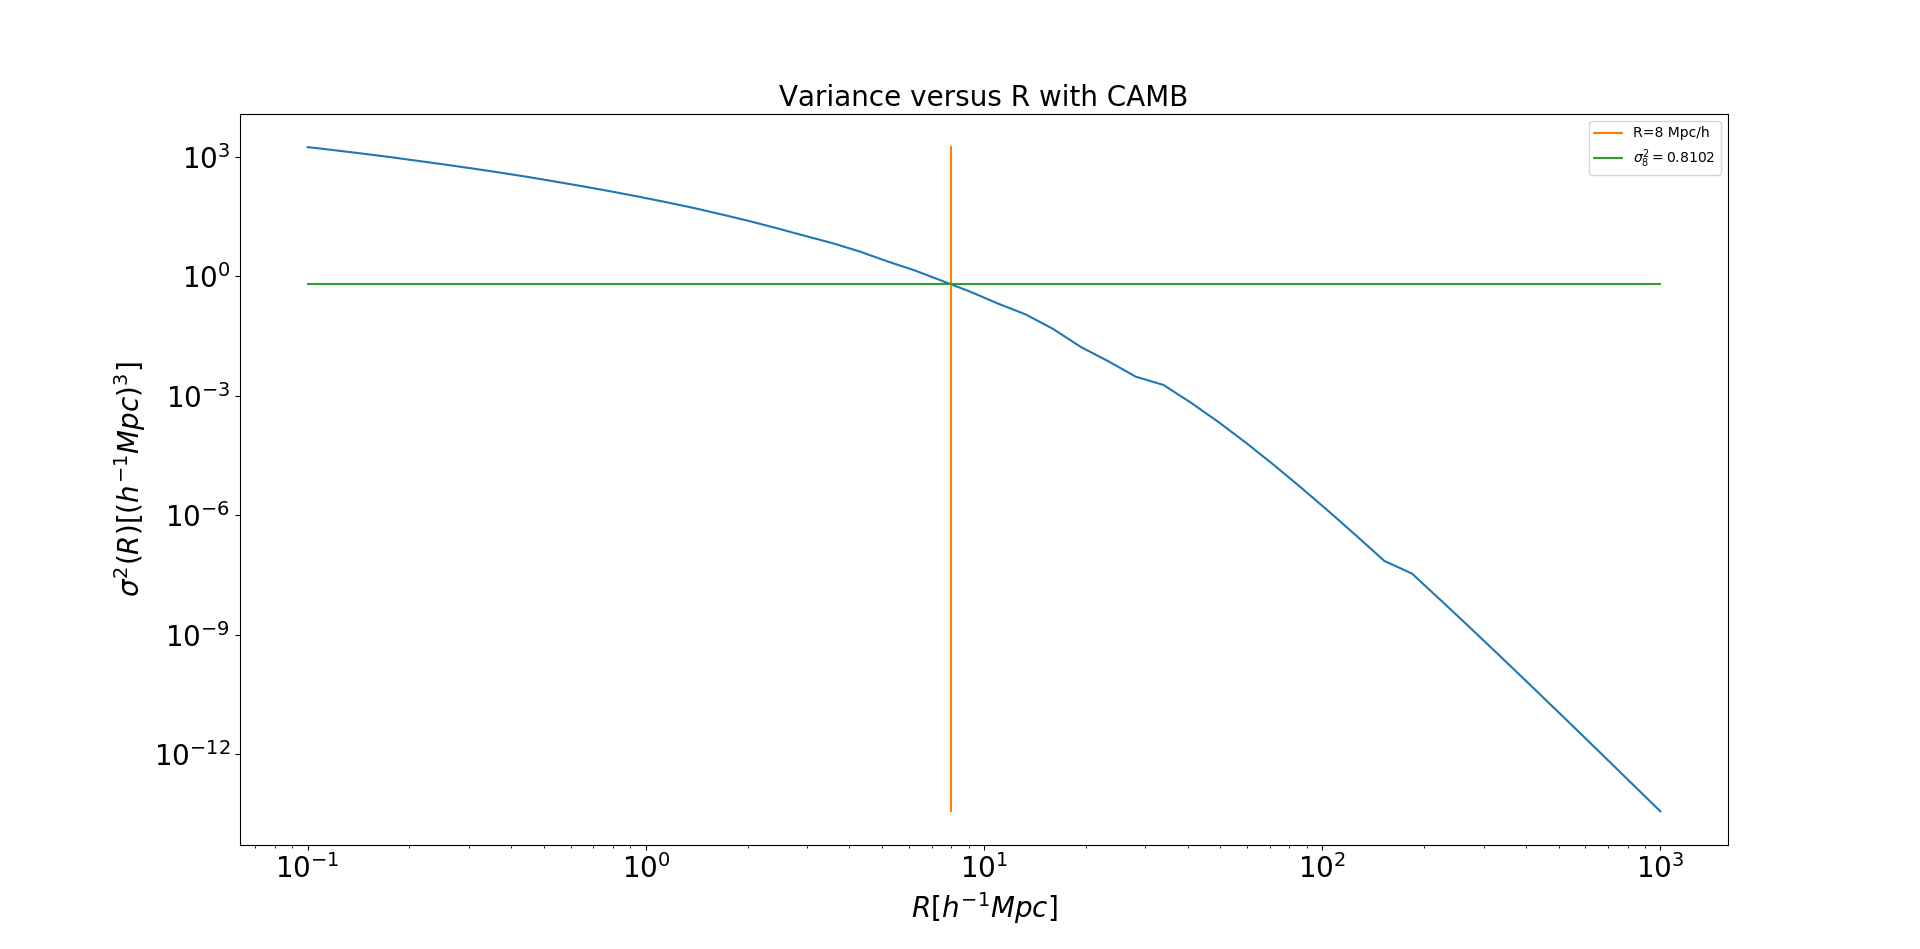
\includegraphics[width=\paperwidth]{Var_vs_R CAMB #5.png}}
	%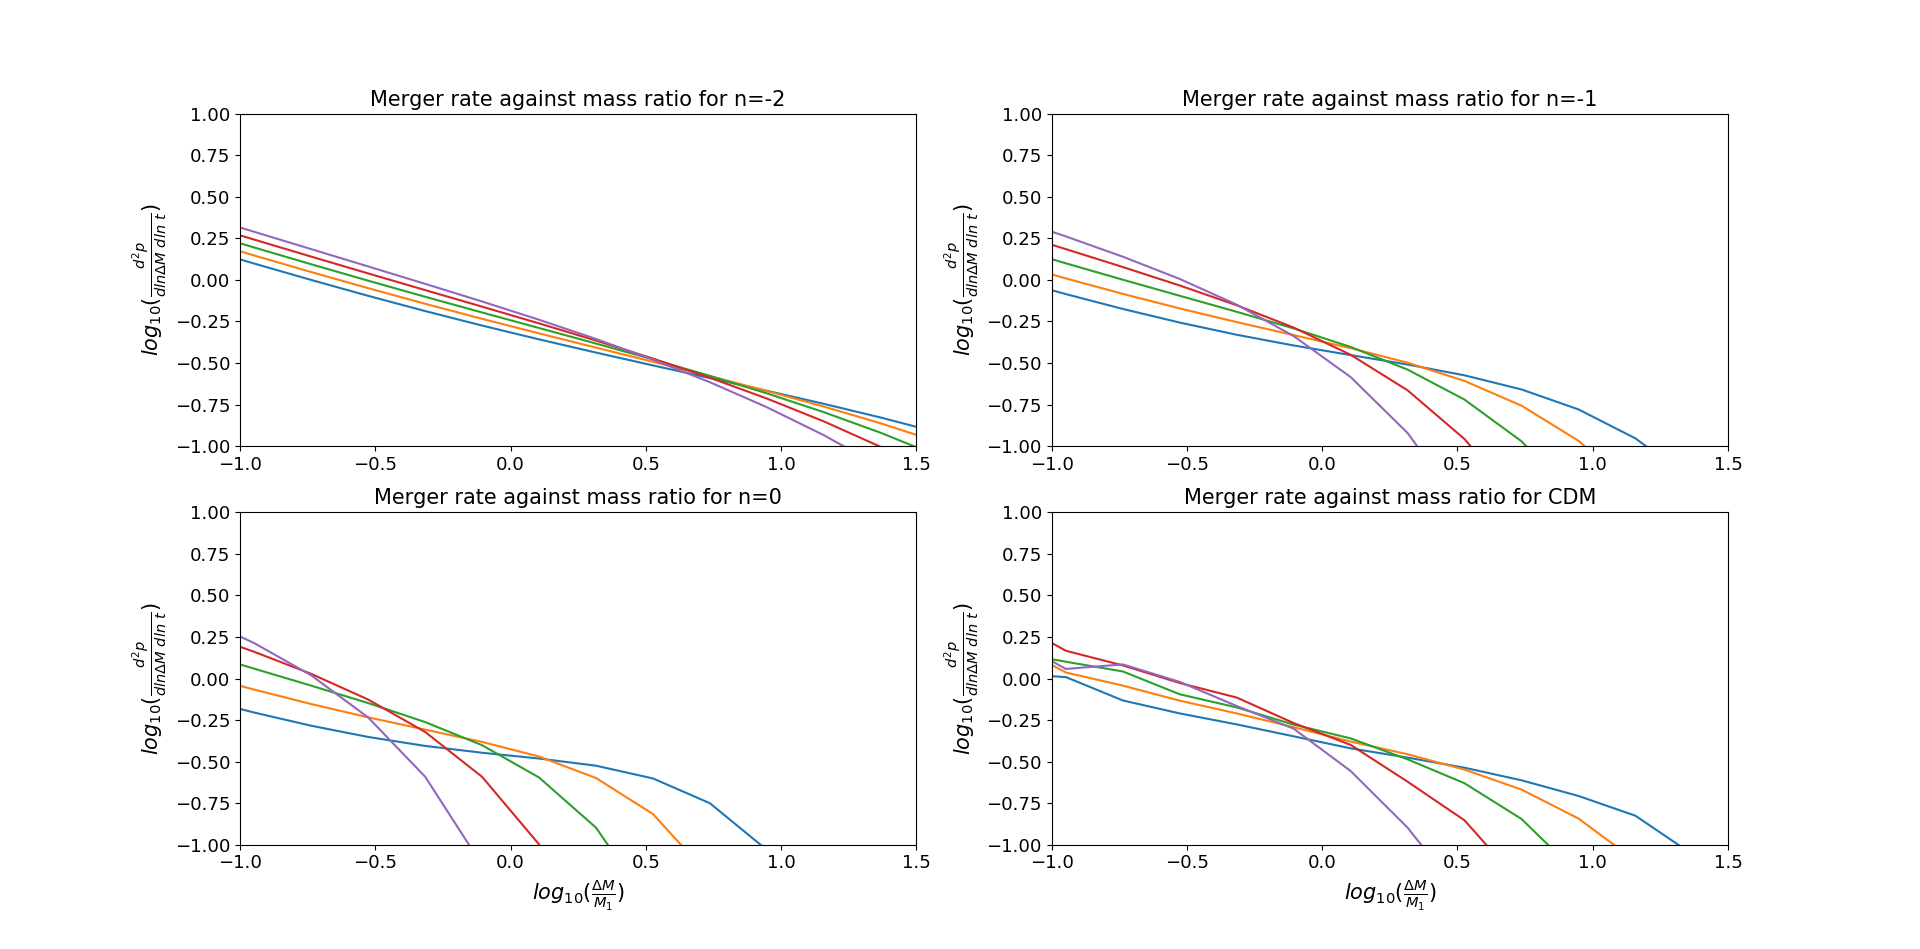
\includegraphics[\textwidth]{Merger_Rate #5.png}
\caption{Variance of a dark matter halo smoothed density vs its effective radius using the standard cosmological parameters obtained by the Planck mission}
\label{Variance Figure}
\end{figure}

We can observe first that, as expected, the variance is monotonically decreasing with the radius. We highlited the $\sigma_8$ value : the value of $S$ for $R =$\SI{8}{\per \h\mega\parsec}. It is a cosmological parameter which is tracer of the structures formation. We renormalized our results so that our variance would match the cosmological parameter.

Once we obtained the variance, we used it to derive the merger rate in equation \ref{MERGER RATE CALC 2} and reproduced a result obtained by Lacey and Cole\cite{LaC}, and obtained the Figure \ref{Merger Rate}. In all the plots, we considered $\Omega_0 = 1$, which leads to $\frac{d \ ln \delta_c}{d \ ln \ t} = -\frac{2}{3}$, and a spherical collapse lead to $\delta_c = 1.69$.

\begin{figure}
\makebox[\textwidth]{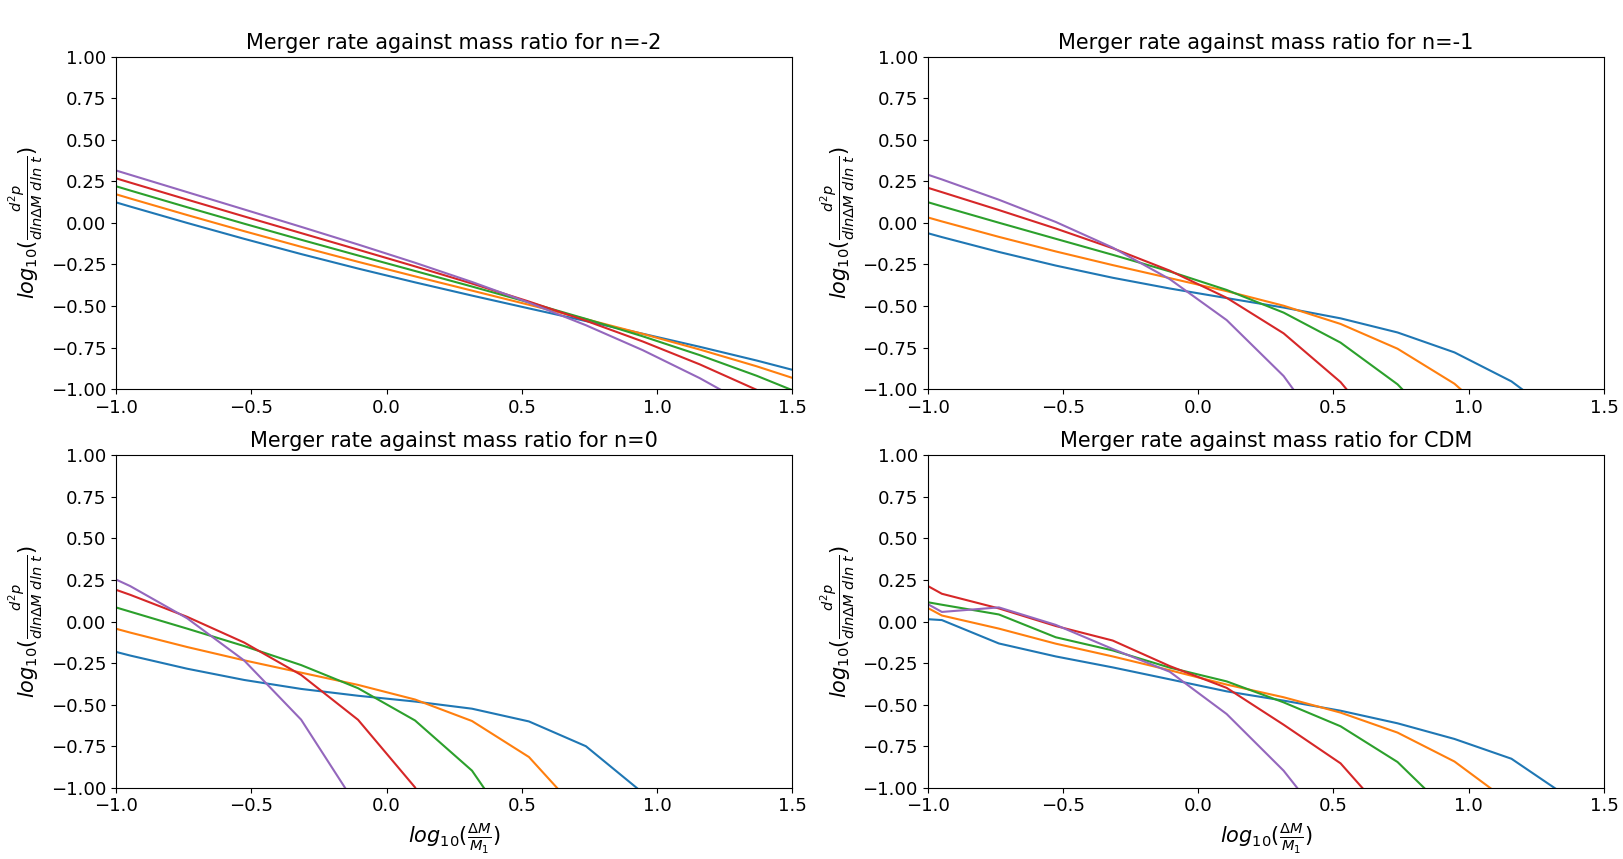
\includegraphics[width=\paperwidth]{Merger_Rate_cropped_#5.png}}
	%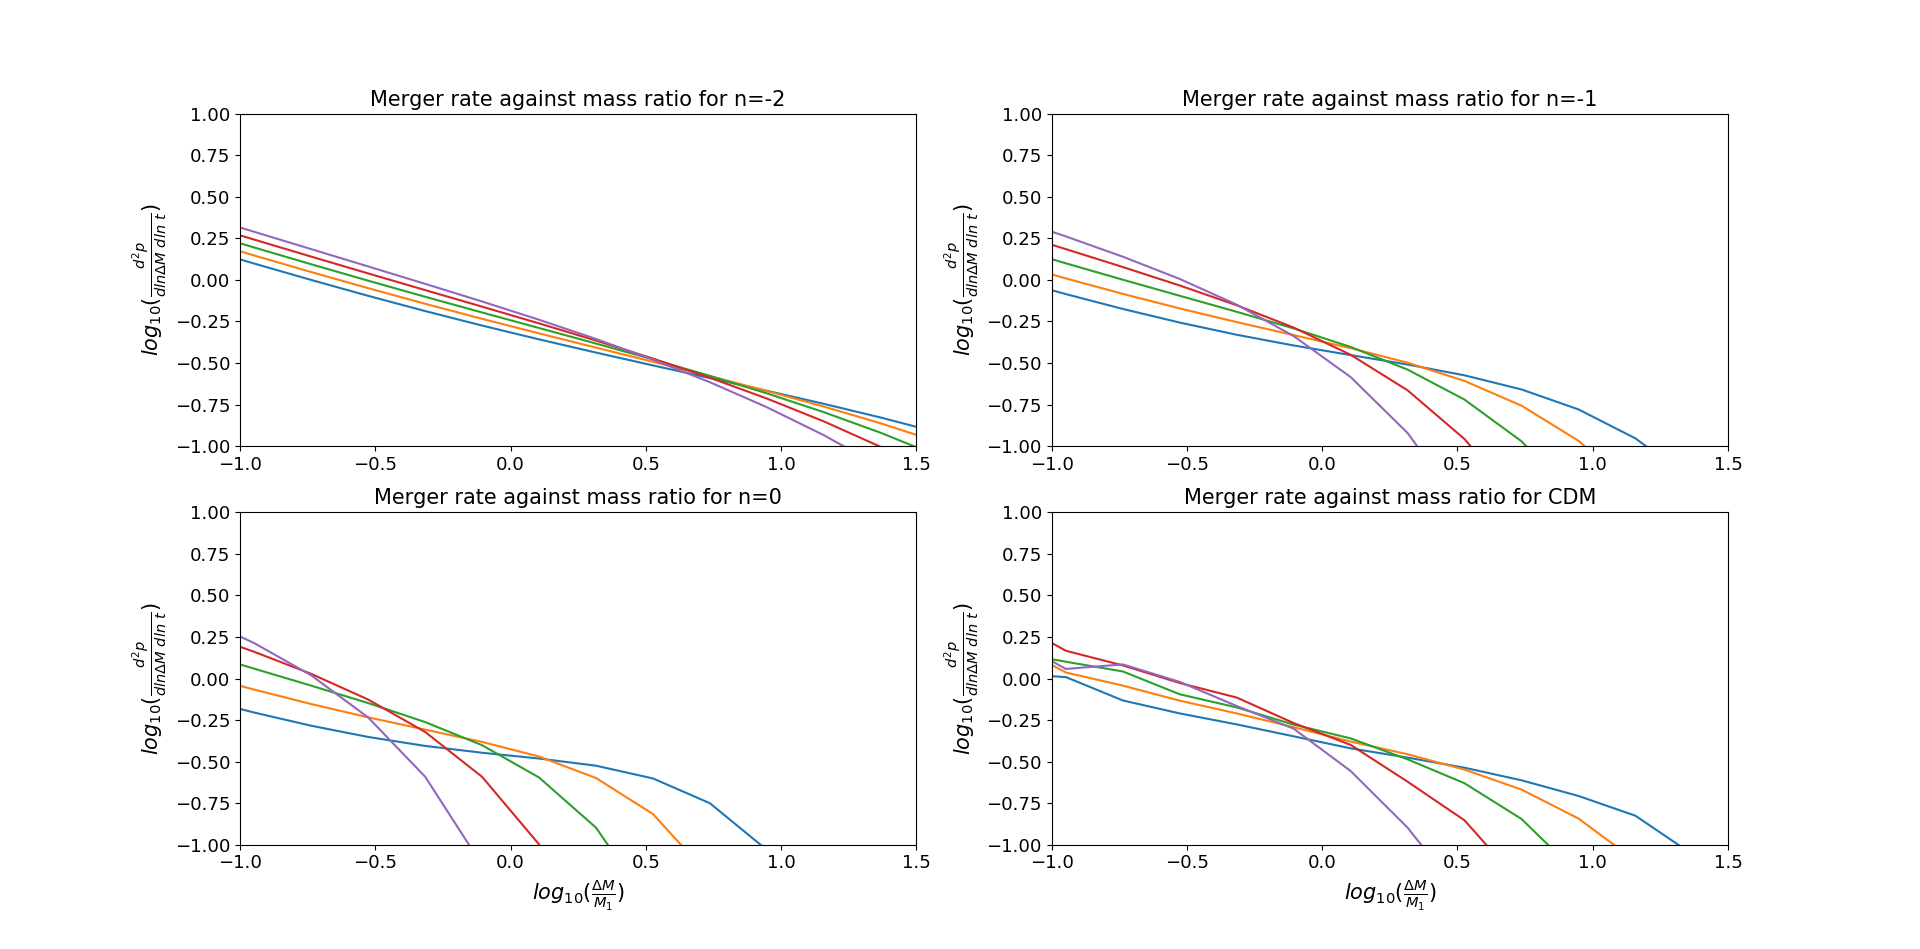
\includegraphics[\textwidth]{Merger_Rate #5.png}
\caption{Merger rate calculation for three toy models and the cosmological paradigm at bottom-right. The different curves correspond in each plot to different masses $M_1 = \frac{1}{2}, 1, 2, 4 or 8 M_\ast$} with $M_\ast = 5.10^{12} M_\odot$
\label{Merger Rate}
\end{figure}


The three first plots, both top and bottom left, correspond to toys models for which we took a power law for the mass distribution $S(M) = 10^{-6} M^{-\frac{n+3}{3}}$.
The last plot corresponds to the standard $\Lambda$ Cold Dark Matter model of cosmology.

We can observe merger with very small halos compared to the halo with mass $M_1$ dominates the merger rate, which also confirm the fact that small halos will tend to disappear with time.
We can also observe the standard cosmological model to be very close to the $n=-1$ power law, so we may use it for further studies as a first approximation for the CDM model.

\newpage
\section*{Conclusion}

Dark matter halos one of the most prominent matter structure of the universe. Their involvement in the formation and evolution of galaxies and their role as a large structure of the universe could help understand better our universe.

Our study focused on the mass distribution of dark matter halos, how it was studied in the Press-Schecter model or the Excursion Set Theory, and the merger rate we can deduce from this last theory.

In addition to our presentation of the theory, it is possible to have a path integral approach to the theory. The Excursion Set Theory can also be used as a base to study non-Gaussianities, predicted by inflation models.

Dark matter halos are usually studied using an empirical universal model for their density called Navarro-Frank-White (NFW). It is possible however to study dark matter halo under another approach which is the sparsity : the ratio of mass contained in two virtual spheres of different radius.
The focus would then be on the halo mass distribution, and the Excursion Set Theory could then be used as a basis.


Finally, we intended to present different merger rates plot for different dark energy models and compare the influence of dark energy on the dark matter halos, but we were not able to perform the study before the finalization of this report.


\section*{Acknowledgements}

I want to thank Pier-Stefano Corasaniti for his help and advices during the internship and the entire cosmology team from the Laboratoire Univers et Théories.

\bibliographystyle{plain}
\bibliography{source}

\newpage
\section*{Annex}


\subsection*{Power spectrum}
\label{Power spectrum Txt}
The primordial perturbations density fluctuations, density fluctuations at very early times, are predicted to be described by homogeneous Gaussian random field. We then have their average to be null :

\begin{equation}
\langle \delta (\textbf{x}) \rangle = 0
\end{equation}

By considering statistical homogeneity and istropy, one can also show the two point function to be in the form :
\begin{equation}
\label{Power Spectrum}
\langle \delta (\textbf{x}) \delta (\textbf{x} + \textbf{r}) \rangle = \int^{\infty}_{-\infty} dln \ k \Delta^2 (k) sinc(kr)
\end{equation}

With :
\begin{itemize}
    \item $k = \mid \textbf{k} \mid$
    \item $r = \mid \textbf{r} \mid$
    \item $\Delta^2 (k) = \frac{k^3 P(k)}{2\pi^2}$
    \item $\langle \widetilde{\delta} (\textbf{k}_1) \widetilde{\delta} (\textbf{k}_2) \rangle = (2\pi)^3 \delta_D (\textbf{k}_1) + \textbf{k}_2) P(k_1)$
    \item $\widetilde{\delta} (\textbf{k})$ the Fourier transform of the density fluctuation 
\end{itemize}

The quantity $P(k)$ is called \textit{power spectrum} and it can be related to the observations. The power spectrum can be seen as a direct probe to study cosmology models and test them.







% Objective - Assemblage de la masse des halos et leur structures interne
% Role centrale de la fonction de masse par le biais du Excursion Set
% Calclue M(z) pour different overdensite


\end{document}